\documentclass[border=5pt, multi, tikz]{standalone}
\usepackage{tkz-graph}
\usetikzlibrary{arrows}
\begin{document}
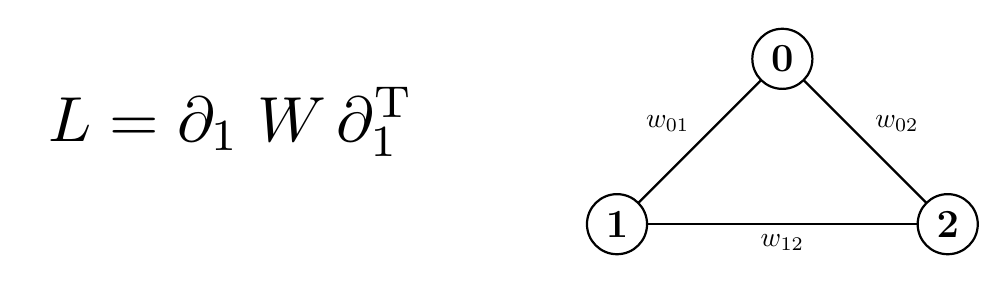
\begin{tikzpicture}[scale=.7,-,>=stealth',shorten >=0pt,thick]
\SetGraphUnit{3} 
\tikzset{VertexStyle/.style = {draw,circle,thick,
                               minimum size=.6cm,
                               font=\Large\bfseries},thick} 
\Vertex{0} \SOWE(0){1} \SOEA(0){2} 
\Edges(2,1,0) \Edge(2)(0)

\path[every node/.style={auto}]    (1) to node {$w_{01}$} (0)
                                       to node {$w_{02}$} (2)
                                       to node {$w_{12}$} (1);

\node[scale=2.3] at (-10,-1.15){$L = \partial_1 \; W\, \partial_1^{\mathrm T}$};
\end{tikzpicture} 
\end{document} 